\documentclass[numbers=noenddot,12pt,a4paper]{scrartcl}
\usepackage[greek,ngerman]{babel}
\usepackage[T1]{fontenc}
\usepackage[utf8]{inputenc}
\usepackage{fullpage}
\usepackage{libertine}
\usepackage{ziffer}
\usepackage{graphicx}
\usepackage{units}
\usepackage[infoshow]{tabularx}
\usepackage{amsmath}
\usepackage{amssymb}
\usepackage{wrapfig}
\usepackage{esint}
\usepackage{float}
\usepackage{wrapfig}
\usepackage[font=small]{caption}
\usepackage{subcaption}
\usepackage{lscape}
\usepackage{hyperref}

\renewcommand{\thefigure}{Abb. \arabic{figure}}

\captionsetup[wrapfigure]{name=}
\captionsetup[figure]{name=}
\newcommand{\degree}{^\circ}
\newcommand{\diff}{\textnormal{d}}
\newcommand{\tenpo}[1]{\cdot 10^{#1}}
\newcommand{\greek}[1]{\greektext#1\latintext}
\newcommand{\ix}[1]{_\text{#1}}
\newcommand{\imag}{\mathbf{i}}
\newcommand{\tilt}[1]{\textit{#1}}
\newcommand{\grad}[1]{\textit{grad}\left(#1\right)}
\newcommand{\divergenz}[1]{\textit{div}\left(#1\right)}
\newcommand{\euler}{\mathnormal{e}}
\newcommand{\sgn}[1]{\text{sgn}\left(#1\right)}

\title{Protokoll: Chaotisches Pendel}
\author{Tom Kranz, Philipp Hacker}
\date{\today}

\begin{document}
%\setcounter{page}{2}
%\setcounter{section}{1}
\maketitle
\begin{center}
Betreuer: Thomas Schumann (Bernd Pompe)\\
Versuchsdatum: 28./29.10.2014\\
\begin{table}[H]
\centering
Note:
\begin{tabularx}{1.5cm}{|X|}
\hline \\ \\
\hline
\end{tabularx}
\end{table}
\end{center}
\vspace*{\fill}
\tableofcontents
\vfill
\newpage
\section{Einleitung}
Der Begriff Chaos beschreibt den Zustand völliger Unordnung und Verwirrung. In der mathematischen Physik ist die \tilt{Chaostheorie} das Feld der nichtlinearen Dynamik, in welcher deterministische Systeme empfindlichst von den Anfangsbedingungen beeinflusst werden.\\
Dieses moderne Feld der Physik bzw. Mathematik wurde durch den von Henri Poincarè gefundenen Lösungsansatz für die Stabilität des Sonnensystems geschaffen. Erst die im letzten Jahrhundert verbesserte Mathematik der Numerik machte es möglich, fälschlich als Ausnahmen angesehene Phänomene, wie Turbulenzen, Dreikörperprobleme o. ä., näherungsweise zu berechnen.\\
Allgemein hin ist das Prinzip des Chaos heute bekannt durch die Metapher des Schmetterlingseffektes beim Wetter.\\
In dem im Folgenden beschriebenen Versuch werden die Prinzipien von nichtlinearer Dynamik am Beispiel eines periodisch erregten Pendels nachvollzogen. Qualitativ sollen so Begrifflichkeiten wie \tilt{Bifurkation}, \tilt{merkwürdiger Attraktor} oder \tilt{Vorhersagehorizont} beobachtet und näher gebracht werden.
\section{Physikalische Grundlagen}
Im Allgemeinen wird die Dynamik eines Systems durch eine Bewegungsgleichung, deren Anfangsbedingungen und die daraus resultierende Trajektorie im Phasenraum vollständig beschrieben. Für beidseitig deterministische Systeme lässt sich damit \tilt{an die Vergangenheit erinnern} und die Zukunft voraussagen (für $t\in\left[-\infty,\infty\right]$).\\
Für reale, chaotische Prozesse sind die Anfangsbedingungen jedoch nicht vollständig bekannt und diese Abweichung, in Form einer kleinen Störung, wächst im zeitlichen Mittel exponentiell an. Somit ist die Vorhersagbarkeit im Vergleich zu rein theoretischen Systemen stark eingeschränkt. Andererseits kann man bei gedämpften (dissipativen) Prozessen die Trajektorie nach einer gewissen Zeit auf einem sog. \tilt{Attraktor} (Mengen im Phasenraum, welche qualitativ stabile Bewegungen beschreiben) finden.
\newpage
\subsection{Nichtlineare Bewegungsgleichung}
\begin{wrapfigure}[18]{ro}{0.33\textwidth}
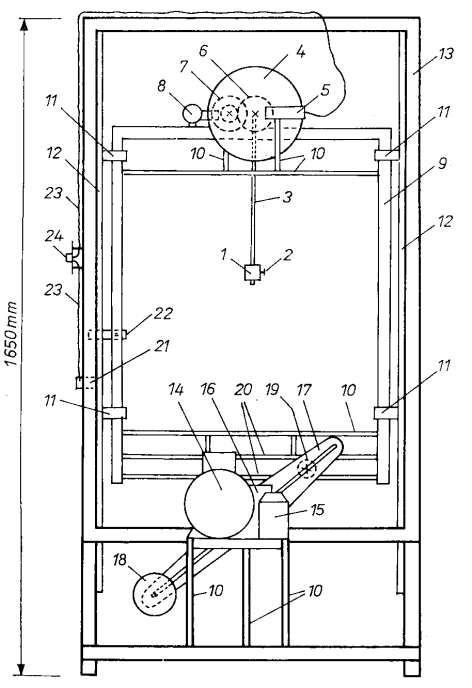
\includegraphics[width=0.39\textwidth]{pendel.png}
\caption{Aufbau, frontales Schema}
\label{img:aufbau}
\end{wrapfigure}
Sei für das ungedämpfte, harmonische Pendel, ohne Erregung im Schwerefeld der Erde, $x(t)$ der Auslenkwinkel im bereich $\left[-\pi; \pi\right]$, $y(t)$ die Winkelgeschwindigkeit (1. totale Ableitung von $x$ nach der Zeit), das Trägheitsmoment $J$, die Masse $m$ und der Abstand zum Schwerpunkt $l$, so gilt
\begin{align}
J\cdot \frac{\diff^2 x}{\diff t^2}+m\cdot g\cdot l\cdot  \sin\left(x\right)=0
\end{align}
für die exakte nichtlineare Bewegungsgleichung.\\
Für die Eigenkreisfrequenz folgt
\begin{align}
\omega_0=\sqrt{\frac{mlg}{J}} \, . \label{eq:freq}
\end{align}
Das Gesamtträgheitsmoment des chaotischen Pendels setzt sich aus den einzelnen Trägheitsmomenten der folgenden Bauteile zusammen: Winkelcodescheibe, Aluminiumscheibe der Wirbelstrombremse (durch Übersetzung das 15-fache!), Zahnkränze, Pendelkörper der Masse $m_K$; Höhe $h_K$ und Pendelstab.
\begin{figure}[H]
\centering
\begin{subfigure}[b]{0.3\textwidth}
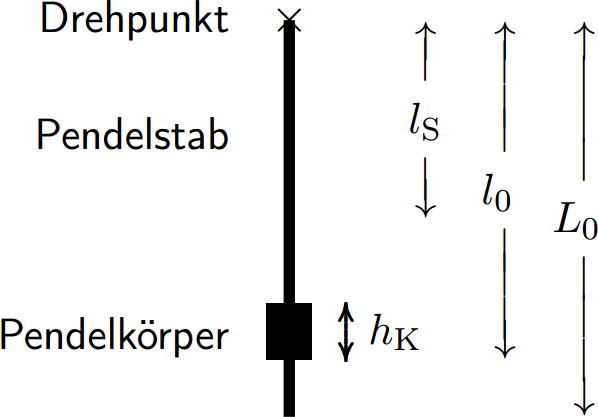
\includegraphics[width=\textwidth]{lnull.png}
\caption{$l_0$, $L_0$, $l_s$} \label{img:lnull}
\end{subfigure}
\begin{subfigure}[b]{0.3\textwidth}
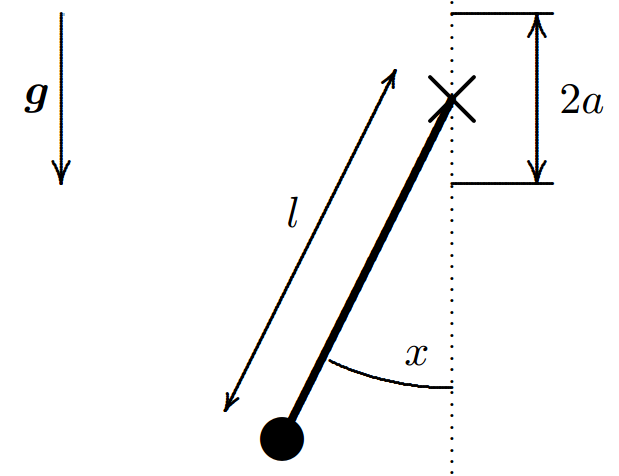
\includegraphics[width=\textwidth]{auslenkung.png}
\caption{Auslenkungsschema} \label{img:auslenkung}
\end{subfigure}
\caption{Längenabmessungen} \label{img:abmessungen}
\end{figure}
Kennt man jedoch das Trägheitsmoment an der Stelle $l_0=L_0$ (siehe Abb. (\ref{img:lnull})), so lässt sich schreiben
\begin{align}
J(l_0)=J(L_0)-m_K\left(L_0^2-l_0^2-h_K\left(L_0-l_0\right)\right) \, . \label{eq:träg}
\end{align}
Für den Abstand $l_S$ zum Massenschwerpunkt des Pendels gilt
\begin{align}
l(l_0)=\frac{m_S\cdot l_S + m_K \cdot \left( l_0- \frac{h_K}{2}\right)}{m_S+m_K} \label{eq:schwer}
\end{align}
Geht man mit (\ref{eq:schwer}) und (\ref{eq:träg}) in (\ref{eq:freq}), so erhält man
\begin{align}
\omega_0(l_0)=\sqrt{\frac{\left(m_S\cdot l_S+m_K\left(l_0-\frac{h_K}{2}\right)\right)\cdot g}{J(L_0)-m_K\cdot \left(L_0^2-l_0^2-h_K\cdot\left(L_0-l_0\right)\right)}}
\end{align}
\subsubsection{Parametrische Erregung}
Versteht man die getriebene, periodische Erregung $h(t)=-a\cdot \cos\left(\omega^\prime t\right)$ durch den Schlitten auf dem der Pendelkörper fährt als zu addierende Beschleunigung zur Erdanziehung, so kann man schreiben
\begin{align}
J\frac{\diff y}{\diff t}+ml\sin\left(x\right)\left(g+\frac{\diff^2 h}{\diff t^2}\right)=J\frac{\diff y}{\diff t}+ml\sin\left(x\right)\left(g+a\cdot \omega^{\prime 2}\cdot \cos\left(\omega^\prime t\right)\right)=0 \label{eq:err}
\end{align}
\subsubsection{Dämpfung}
Das durch die Wirbelstrombremse erzeugte Dämpfungs-/Bremsdrehmoment wird über ein Getriebe der Übersetzung $V$ (100:15) auf das Pendel übertragen. Hinzu kommt die nicht justierbare Dissipation durch Reibungen im Lager und mit der Luft.\\
Die Dämpfung enthält somit einen konstanten Term und einen, der mit der Winkelgeschwindigkeit bzw. dem magnetischen Fluss (somit dem Strom $I$) geht.
\begin{align}
M_D=b_0\cdot\sgn{y}+b_1\cdot y \label{eq:dämpf}
\end{align}
\subsubsection{Normierung}
Zur übersichtlicheren Darstellung wird die Bewegungsgleichung, welche sich jetzt aus (\ref{eq:dämpf}) und (\ref{eq:err}) zusammensetzt, durch folgende Normierungen bzw. dimensionslose Variablen vereinfacht:
\begin{align}
\frac{\diff y}{\diff \tau}=\dot y &\hspace{1.5cm} \frac{\diff x}{\diff \tau}=\dot x=y\\
\text{Zeit: } \, \tau=\omega_0 t &\hspace{1.5cm} \text{Erregerfrequenz: } \, \Omega(l_0)=\frac{\omega^\prime}{\omega_0} \\
\text{konst. Dämpfung: } \, \beta_0(l_0)=\frac{b_0}{J\omega_0^2} &\hspace{1.5cm} \text{normierte Dämpfung: } \, \beta_1(l_0, I)=\frac{b_1}{J\omega_0} \\
\text{normierte Amplitude: }& \, \alpha(a)=\frac{\omega^{\prime 2}\cdot a}{g} \, .
\end{align}
Die Bewegungsgleichung, die man damit erhält, ist stark nichtlinear. Sie lautet:
\begin{align}
\dot y+\beta_0\cdot\sgn{y}+\beta_1\cdot y+ \left(1+\alpha\cdot\cos\left(\Omega \tau\right)\right)\cdot\sin\left(x\right)=0 \, .
\end{align}
\subsection{Beschreibung des chaotischen Prozesses}
\subsubsection{Regime der Bewegung}
Die oberfl\"achliche Qualit\"at und Charakteristik einer Bewegung kann allgemein als Regime bezeichnet werden. F\"ur bestimmte Anfangsbedingungen der Variablen $\left(x_{0};y_0\right)$ und Werte f\"ur die Parameter stellt sich nach einer gewissen Einschwingzeit asymptotisch ein Bewegungsregime ein.\\
Rotationsbewegungen werden solche genannt, deren $\sgn{y}=const.$ ist bzw. die permanent in eine Richtung schwingen. Sie sind charakteristisch f\"ur grob{\ss}e $y_0$. Ist die Auslenkung \"uber beliebig gr\"o{\ss}e $\tau$ hinweg bescher\"ankt, so spricht man von einer Librationsbewegung. Alle anderen Bahnen im vollst\"andigen Phasenraum geh\"oren zu den transient chaotische Bewegungen. Die zeichnen sich durch ihre starke Abh\\"angigkeit von den Anfangsbedingungen aus. Es ist m\"oglich, Einschwingzeiten von mehreren hundert Erregerperioden verstreichen zu lassen, um dann eine qualitative Bewegungs\"anderung zu beobachten.
\subsubsection{Stroboskopisches Phasenraumportrait} \label{sec:strobo}
Der 3-dim. Raum, welcher die Bewegung des Pendels zu jeder Zeit und in jedem Zustand einschlie{\ss}t, hei{\ss}t vollst\"andiger Phasenraum. Er wird aus  der Ausrenkung $x(\tau)$, der Winkelgeschwindigkeit $y(\tau)$ und der Zeit $\tau$ aufgespannt.  Es reicht hierbei jedoch, das Produkt aus den Intervallen $\left[-\pi;\pi\right]$ f\"ur die Auslenkung, $\left[-\infty;\infty\right]$ f\"ur die Winkelgeschwindigkeit und $\left[0;2\pi\right]$ f\"ur die normierte Erregerphase zu betrachten. \\
Die Darstellung von Punkten der Trajektorie, welche zu gleichwertigen Zeiten aufgenommen wurden, k\"onnen zusammen als zweidimensionales, \tilt{stroboskopisches Phasenraumportrait} aufgefasst werden. Dieser ist auf die Auslenkung und die Winkelgeschwindigkeit reduziert.
\subsubsection{Attraktoren}
Attraktoren sind Punktmengen im Phasenraum dissipativer Systeme, auf welche transiente Bewegungen asymptotisch zulaufen. Sie beschreiben stabile Zust\"ande. Bez\"uglich des \tilt{Lebesgue-Ma{\ss}} sind sie Nullmengen: unter dem Strom im Phasenraum schrumpft das Volumen \"uber die Zeit. Dies kommt durch die Divergenz von
\begin{align}
\divergenz{\dot x; \dot y}=-\beta_{0}\cdot\delta\left(y\right)-\beta_{1}
\end{align}
zum Ausdruck. Somit kann die Einschwingzeit, die f\"ur das Anlaufen des Attraktors durch die Bewegung ben\"otigt wird, unendlich lange werden. Diese Zeit ist jedoch f\"ur den Experimentator beendet, wenn die Trajektorie n\"aher am Attraktor liegt, als die Messaufl\"osung die Darstellung zul\"asst. Kompliziertere Gebilde dieser Art hei{\ss}en \tilt{fraktal} und deren Attraktoren \tilt{seltsam} (nach \tilt{B Mandelbrot}).
\subsubsection{Bifurkationsdiagramme}
\begin{figure}[h]
\centering
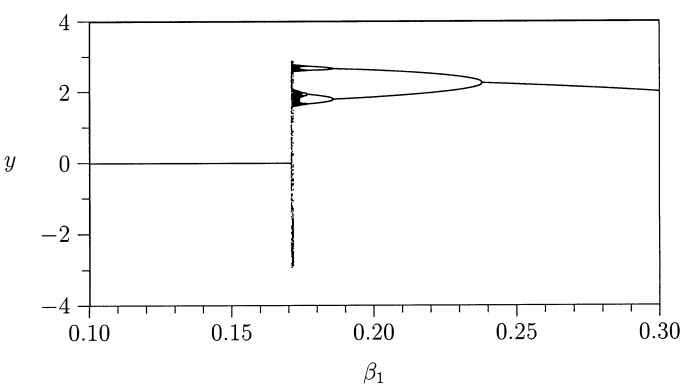
\includegraphics[width=0.7\textwidth]{bifur.png}
\caption{Winkelgeschwindigkeit $y$ über Parameter $\beta_1$} \label{img:bifur}
\end{figure}
Eine stroboskopische Darstellung der Auslenkung oder der Winkelgeschwindigkeit gegen einen Parameter der Bewegung nennt man Bifurkationsdiagramm (\ref{img:bifur}). In diesem kann man die qualitativen Bewegung\"anderungen (\tilt{Bifurkationen}) in Abh\"angigkeit des verwendeten Parameters ablesen. Beispielsweise l\"asst sich so der Verlauf der Periodizit\"at der Pendelbewegung bei externer Erregung verfolgen (``Rotations-Einer'' $\rightarrow$ ``Rotations-Zweier'' $\rightarrow \, \dots$ Chaos).
\subsubsection{Vorhersagehorizont}
Mit Hilfe des \tilt{Lyapunov-Exponenten} $\lambda$ kann man, bei einer Messgenauigkeit $\varepsilon$ für eine Bewegung auf einem Attraktor des Durchmessers $\epsilon$, den Prozess qualitativ vorhersagen, solange wie
\begin{align}
\varepsilon\cdot\euler^{\lambda\cdot \tau}\lesssim\epsilon
\end{align}
gilt. Für den \tilt{Lyapunov-Exponenten} und den Vorhersagehorizont (in der Zeit) gilt, bei einer kleinen Störung $\xi$ der Trajektorie, folgendes:
\begin{align}
\overline{||\xi(\tau)||}=||\xi(0)||\cdot\euler^{\lambda\tau} \\
\tau_{vor}\approx\frac{1}{\lambda}\cdot\ln\left(\frac{\epsilon}{\varepsilon}\right) \, .
\end{align}
Es entfernen sich zwei Trajektorien, ungestört und gestört, im zeitlichen Mittel exponentiell. Somit ist die Vorhersagbarkeit stark eingeschränkt. Messfehler, welche für die Anfangsbedingungen gemacht werden, zerstören somit die Erwartungen an den Prozess. Für chaotische Bewegungen ist $\lambda>0$.\\
Mit $\lambda$ kann außerdem die Informationsmenge $I$ berechnet werden, welche proportional (\tilt{Informationsdimension} $D_I$) mit einer Verbesserung der relativen Messgenauigkeit $G=\frac{\epsilon}{\varepsilon}$ geht:
\begin{align}
I&\sim D_I\ln\left(G\right) \\ D_I&=1+\frac{\lambda}{\lambda+\beta_1}
\end{align}
Als Vorhersagehorizont lässt sie auch jene Zeit verstehen, welche benötigt wird, um die Informationen zum Anfangszustand vollständig durch neue zu ersetzen: $\tau_{vor}\cdot\lambda\approx I(G)$.\\
Für $G$ gilt in unserem Versuch $2^{-8}$. 
\begin{align}
\tau_{vor}\approx& \frac{D_I}{\lambda}\ln\left(G\right) \approx\frac{1.8}{\frac{\Omega}{2\pi}}\cdot\ln\left(2^8\right)\approx 10\cdot\frac{2\pi}{\Omega}
\end{align}
Für \underline{$\tau<<\tau_{vor}$} sind die chaotischen Bewegungen aus den Anfangsbedingungen vorhersagbar.
Mit \underline{$\tau\lesssim\tau_{vor}$} wird die Vorhersagbarkeit u.U. stark eingeschränkt.
Ist \underline{$\tau>\tau_{vor}$}, so lässt sich die chaot. Bewegung nicht mehr vorhersagen. Allein ob sie auf einem Attraktor stattfinden wird kann abgeschätzt werden.
\section{Durchführung}
\subsection{Versuchsaufbau}
\begin{wrapfigure}[12]{l}{0.33\textwidth}
\centering
\vspace{-0.5cm}
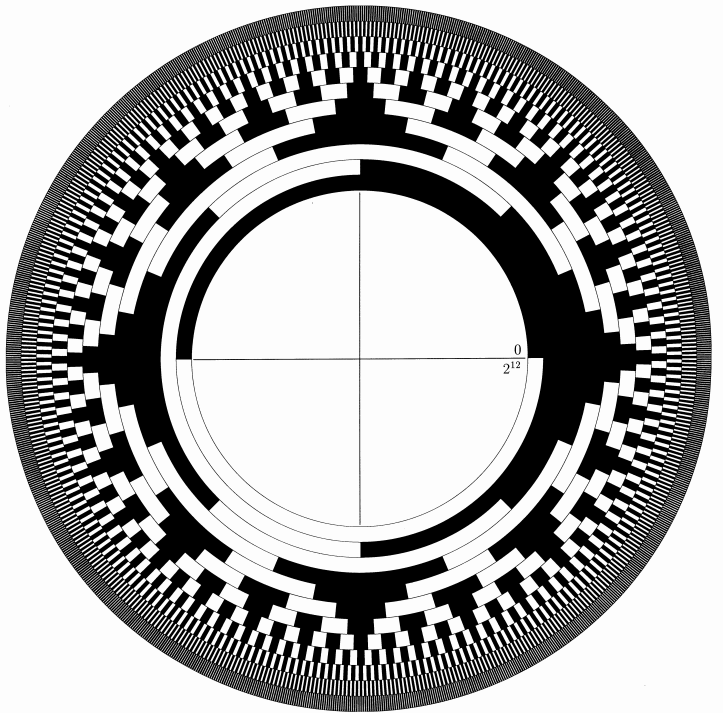
\includegraphics[scale=0.2]{winkelkot.png}
\caption{\tilt{Ein-Schritt-Code}-Scheibe} \label{img:winkelkot}
\end{wrapfigure}
Der Aufbau des Pendels kann in der \ref{img:aufbau} und \ref{img:abmessungen} eingesehen werden.\\
Im Rahmen sind des Weiteren Platinen für Microcontroller (MC) und integrierte Schaltkreise angebracht. Diese werden bei einer konstanten Spannung von $\pm\unit[5]{V}$ betrieben. Sie verarbeiten die, von Photodioden in den Auflicht-Lichtschranken an der Winkelcodescheibe (siehe \ref{img:winkelkot}), erzeugten Signale. Außerdem geben Analog-Digital-Wandler dem Experimentator die Möglichkeit, Phase sowie Auslenkung zu Oszillographieren (\tilt{x-y-Modus}). Außerdem kann die besprochene \tilt{stroboskopische Phasenraumdarstellung} aus \ref{sec:strobo} dadurch realisiert werden, dass am MC ein Neustart des Programms mit Halten eines 2. Knopfes erfolgt. Dabei ändert sich das analoge Signal in der Form, dass die Ausgabe nur noch zeitsynchron mit dem zweiten Durchgang des Schlittens durch die Lichtschranke im unteren Totpunkt der Erregung stattfindet. Zu beachten ist jedoch, dass zum Zeitpunkt der Aufnahme von die Phase der Erregung nicht immer die gleich ist. Die Lichtschranke kann die Durchgangsrichtungen nicht unterscheiden.\\
Die Drehachse wird über ein Getriebe mit einem Verhältnis von 100:15 auf die Wirbelstrombremse übersetzt. Das heißt, dass schon geringe Ströme und somit Flussdichten durch die Aluminiumscheibe ausreichen, um ein signifikantes Verzögerungsmoment hervorzurufen. Der Strom wird von 2 in Reihe geschalteten Netzteilen geliefert.\\
Die Amplitude der, durch einen Elektromotor getriebenen Erregung, sowie die Lage des Pendelkörpers sind variabel. 
\subsection{Ablauf}
Eingangs wird bei abgeschalteter Erregung und unter Änderung des Abstandes des Pendelkörpers von der Drehachse am Oszilloskop (\tilt{Roll-Modus}) die  Schwingungsfrequenz untersucht.\\
Anschließend wird bei sukzessiver Änderung des Parameters Strom im stroboskopischen Phasenraumbild nach der Bifurkation einer Periodenverdopplung gesucht. Beispielsweise kann das der Übergang von einer \tilt{Einer-Periode} zu einer  \tilt{Zweierperiode} (siehe \ref{img:bifur} an $\beta_1\approx$ 0.24) sein. Außerdem wird jeweils eine Messung für ein $\Omega$ gemacht. Die gefundenen Werte werden danach mit denen der numerischen Simulation des bereitgestellten Programms verglichen. Die Amplitude sowie Frequenz der Erregung bleibt konstant.\\
Schließlicht erfolgt nach Einstellung der, in der Anleitung gegebenen Parameter eine Messung zu den Anfangsbedingungen einer bestimmten Erreger-Phasenlage. Hierzu wird die Auslenkung und Winkelgeschwindigkeit zeitabhängig Oszillographiert. Das gewonnene Bild wird wiederum mit der Simulation für die ausgewählten Werte verglichen.
\section{Messungen}
Zuerst wurden die Frequenzen für Schwingungen beliebiger Größe bei ausgeschalteter Wirbelstrombremse und maximalem Abstand des Pendelgewichts gemessen. Die Ergebnisse sind in \ref{img:freq} dargestellt, zusammen mit einer Näherung, die in der Versuchsanleitung vorgeschlagen wurde. Diese Näherung sollte erst ab einer Auslenkung von $\frac{\pi}{2}$ merkliche Abweichungen von der exakten Lösung aufweisen, was mit unserer Messung sehr gut korreliert. Die Messung der Frequenzen erfolgte durch Vermessen der Zeit zwischen zwei Auslenkungsextrema ($\hat{=}\frac{T}{2}$), die der Auslenkung durch Mittelwertbildung der ausgegebenen Spannungen bei diesen Maxima. Der Fehlerbereich hierfür ist großzügig gewählt, nämlich der halbe Unterschied zwischen den beiden Maxima, zuzüglich einer geschätzten Messunsicherheit des Oszilloskops von $\Delta U\approx\unit[30]{mV}$ bei Philipps Messungen, beziehungsweise $\Delta U\approx\unit[3]{mV}$ bei Toms Messungen. Die Diskrepanz erklärt sich durch die Wahl unterschiedlicher Messbereiche. Die Messunsicherheit der Frequenz (das Oszilloskop bot eine Funktion zum "`direkten"' Messen von Frequenzen) haben wir zu $\Delta f\approx\unit[0,03]{Hz}$ geschätzt. Lediglich im Bereich höherer Auslenkungen kommt es zur Abweichung der Näherung von den Messwerten -- aufgrund des eingeschränkten Gültigkeitsbereichs der Näherung entspricht dies aber völlig den Erwartungen. Ein oberflächlicher Vergleich mit der in der Anleitung gegebenen (aber leider nicht näher spezifizierten) Kurve ergibt sogar in diesem Bereich eine Übereinstimmung.
\begin{figure}[H]
	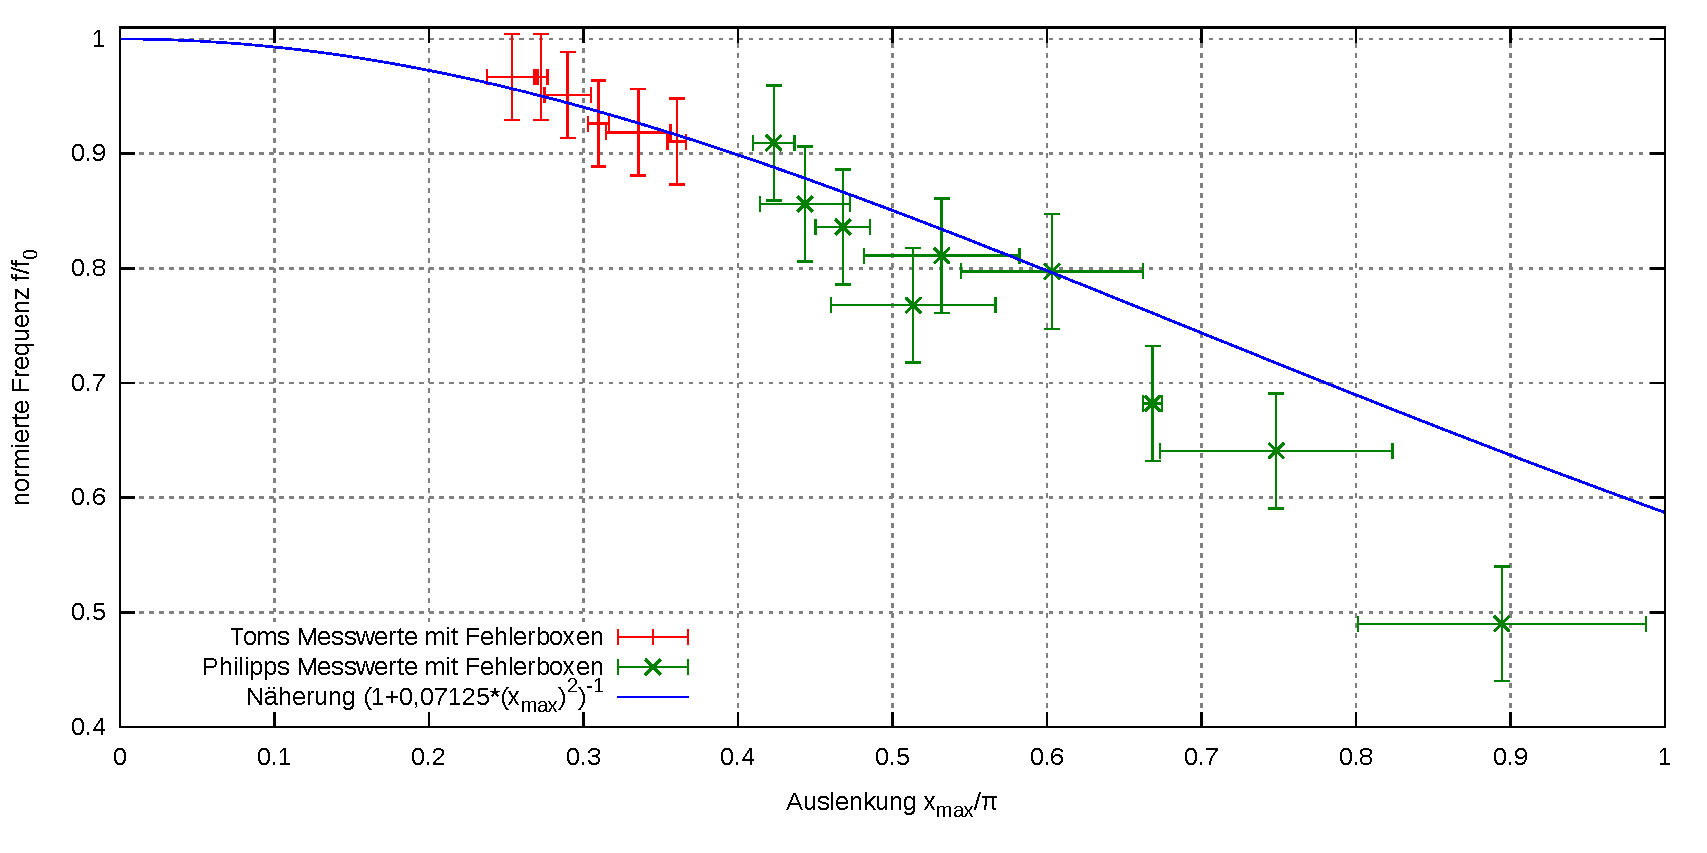
\includegraphics[width=\textwidth]{messwerte/frequenzauslenkung.pdf}
	\caption{Frequenzen der Pendelbewegung bei unterschiedlichen Auslenkungen}
	\label{img:freq}
\end{figure}
Als nächstes wurden Bifurkationen untersucht. Zuerst wurden feste Parameter vorgegeben, das Pendel in ein Rotationsregime getrieben und dann $\beta\ix{1}$ kontinuierlich verändert, bis sich im stroboskopischen Phasenraumbild eine Periodenverdopplung zeigte. Dies wurde für einen ansonsten festen Parametersatz zweimal getan und dann wurde der Abstand des Pendelgewichts von der Drehachse geändert, um $\Omega$ einen neuen Wert zu geben. Nach erfolgreichem Einschwingen im Rotationsregime wurde auch hier wieder $\beta\ix{1}$ kontinuierlich bis zur Periodenverdopplung verändert. Die Ergebnisse zeigt \ref{img:beef}. Unsere Fehlerberechnung stützt sich auf das Gaußsche Fehlerfortpflanzungsgesetz, das wir mit einem CAS auf die funktionalen Zusammenhänge zwischen normierten Parametern und Messgrößen angewendet haben, um letztlich die eingezeichneten Messfehler zu erhalten. Von der Anleitung wurde an dieser Stelle eine Simulation empfohlen, um die Bifurkationsstellen zu verifizieren oder zumindest mit der Simulation zu vergleichen. Da das vorgeschlagene Programm jedoch in unserem Parameterbereich keine auswertbaren Bifurkationsdiagramme geliefert hat, können wir an dieser Stelle leider keinen Vergleich zur Simulation liefern. Da keine Kenntnisse über den Zusammenhang von $\Omega$ und $\beta\ix{1}$ in der Parameterebene bestehen, kann auch kein Rückschluss auf die Qualität der gewonnenen Messwerte gemacht werden. Nichtsdestotrotz beobachteten  wir für die in \ref{img:beef} gezeigten Werte qualitative Bewegungsänderung des Pendels, was den Erwartung aus den Grundlagen gerecht wird.
\begin{figure}[H]
	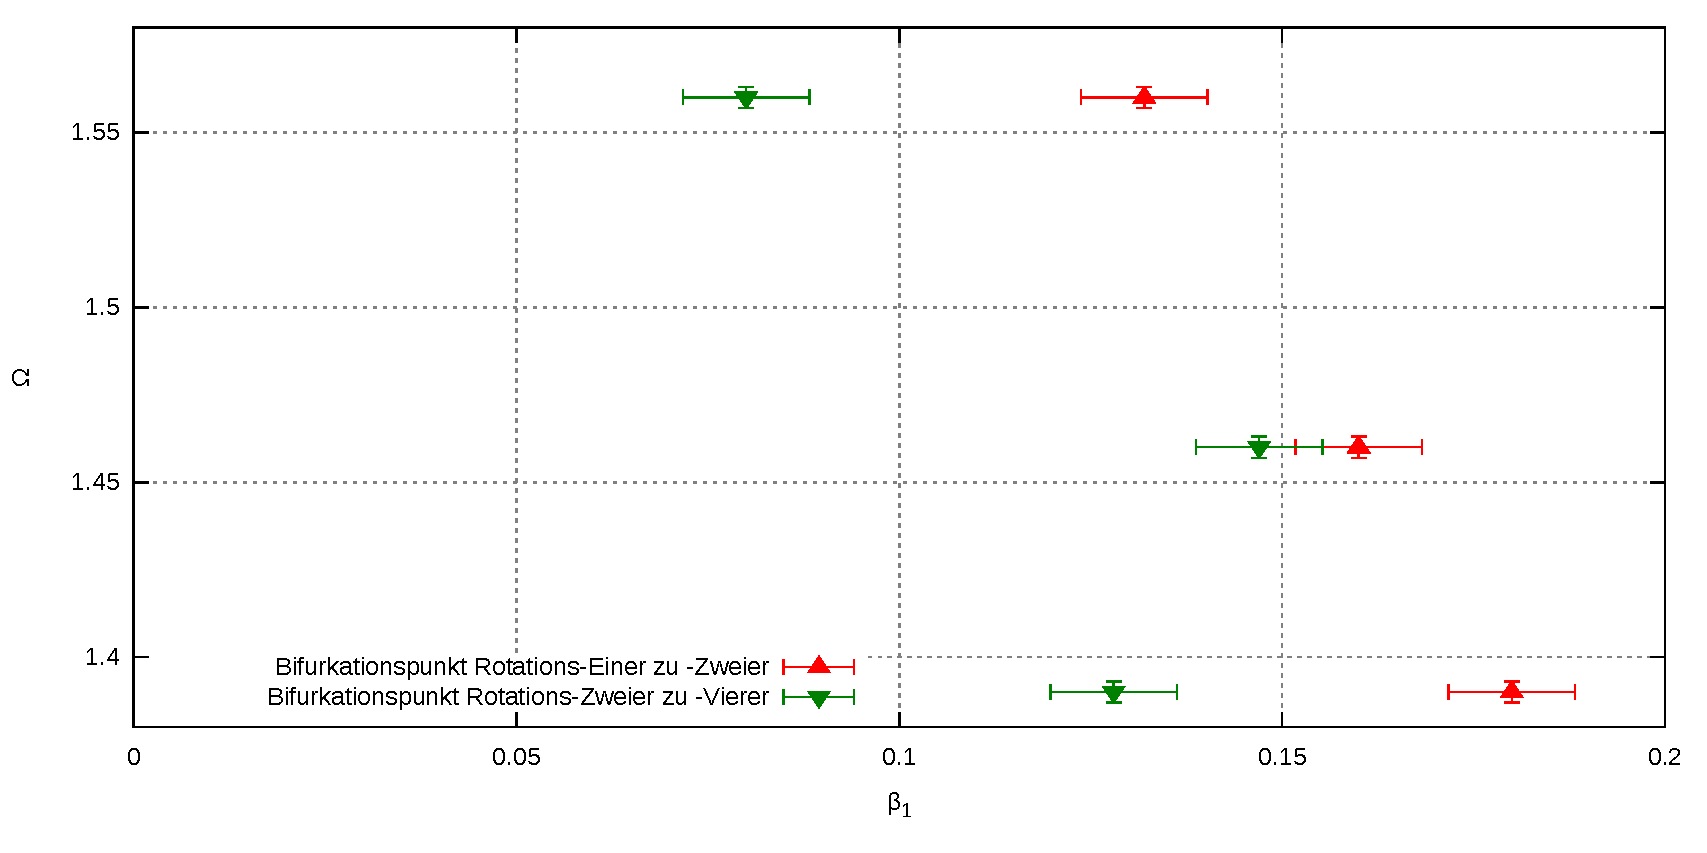
\includegraphics[width=\textwidth]{messwerte/beefurkation.pdf}
	\caption{Punkte in der $(\Omega;\beta\ix{1})$-Parameterebene, bei denen Bifurkationen auftraten}
	\label{img:beef}
\end{figure}
Um Aussagen über den Vorhersagehorizont machen zu können, war es notwendig, zeitsynchron mit der Phase der Erregung die Auslenkung und die Winkelgeschwindigkeit aufzunehmen. Dies war jedoch bei dem gegebenen Versuchsaufbau nicht möglich, weswegen wiederum kein Vergleich zur Simulation angestellt werden konnte. Wir erhielten keine Referenz für die Aussagen über den Vorhersagehorizont.
\section{Quellen}
\url{http://de.wikipedia.org/wiki/Chaos}\\
\url{http://de.wikipedia.org/wiki/Chaosforschung}\\
Versuchsanleitung "`Bifurkation und Chaos(Pendel)"'
\section{Anhang}
Die originalen Messwert-Aufzeichnungen liegen bei.
\end{document}